\documentclass[tikz,border=4pt]{standalone}
\usepackage{tikz}
\usetikzlibrary{calc,positioning,shapes,arrows.meta}
\begin{document}

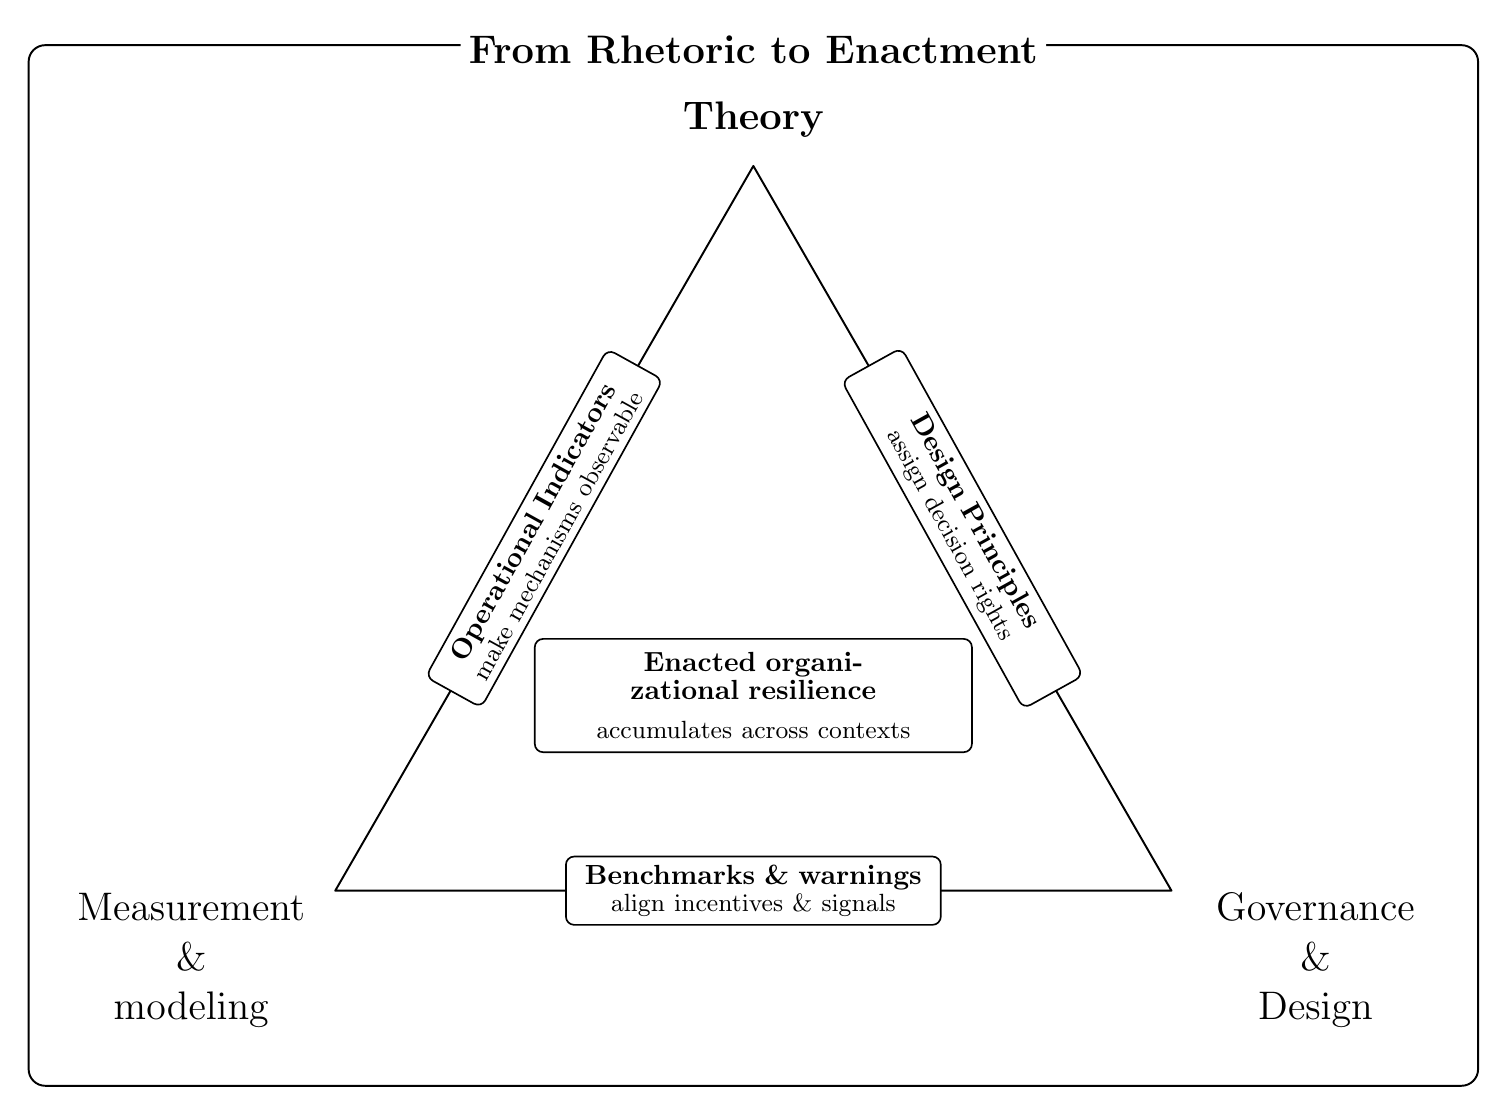
\begin{tikzpicture}[x=1.18cm,y=1.18cm,font=\rmfamily, line cap=round, line join=round]

% ---------- styles ----------
\tikzset{
  frame/.style={draw, rounded corners=6pt, line width=0.7pt},
  tri/.style={draw, line width=0.7pt},
  box/.style={draw, rounded corners=3pt, line width=0.6pt, fill=white, align=center},
  tlabel/.style={font=\bfseries\Large, align=center},
  clabel/.style={font=\Large, align=center},
  small/.style={font=\small},
  tiny/.style={font=\footnotesize},
}

% ---------- canvas coordinates ----------
% Outer frame corners (tightened, with small breathing room around labels)
\coordinate (Fsw) at (-7.80,-5.95);
\coordinate (Fne) at ( 7.80, 5.25);
\coordinate (Fnw) at (-7.80, 5.25);
\coordinate (Fse) at ( 7.80,-5.95);

% Triangle vertices (kept centered in the frame)
\coordinate (Apex) at (0,3.95);
\coordinate (L)    at (-4.5,-3.85);
\coordinate (R)    at ( 4.5,-3.85);

% ---------- outer frame ----------
\draw[frame] (Fsw) rectangle (Fne);

% Title sitting "on" the top border (white background masks the frame line)
\node[box, draw=none, fill=white, text=black, font=\bfseries\Large, inner sep=3pt]
  at (0,5.20) {From Rhetoric to Enactment};

% ---------- main triangle ----------
\draw[tri] (L) -- (Apex) -- (R) -- cycle;

% Vertex labels
\node[tlabel] at ($(Apex)+(0,0.50)$) {Theory};

\node[clabel] at ($(L)+(-1.55,-0.75)$)
  {Measurement\\ \&\\ modeling};

\node[clabel] at ($(R)+(1.55,-0.75)$)
  {Governance\\ \&\\ Design};

% ---------- side mechanism boxes ----------
% Left side (rotated along left edge)
\node[box, rotate=61, text width=4.55cm, inner sep=3.0pt]
  at ($ (L)!0.5!(Apex) $)
  {{\bfseries Operational Indicators}\\[-2pt]
   {\small make mechanisms observable}};

% Right side (rotated along right edge)
\node[box, rotate=-61, text width=4.55cm, inner sep=3.0pt]
  at ($ (R)!0.5!(Apex) $)
  {{\bfseries Design Principles}\\[-2pt]
   {\small assign decision rights}};

% ---------- center box ----------
\node[box, text width=5.2cm, inner sep=5.0pt]
  at (0, -1.75)
  {{\bfseries Enacted organi-}\\[-2pt]
   {\bfseries zational resilience}\\[2pt]
   {\small accumulates across contexts}};

% ---------- bottom box ----------
\node[box, text width=4.55cm, inner sep=3.0pt]
  at (0, -3.85)
  {{\bfseries Benchmarks \& warnings}\\[-2pt]
   {\small align incentives \& signals}};

\end{tikzpicture}
\end{document}